\documentclass[11pt]{article}

% ── Packages ─────────────────────────────────────────────
\usepackage[margin=1in]{geometry}
\usepackage[utf8]{inputenc}
\usepackage[T1]{fontenc}
\usepackage{amsmath,amssymb,amsthm,mathtools}
\usepackage[american]{babel}
\usepackage{enumitem}
\usepackage{booktabs}
\usepackage{array}
\usepackage{longtable}
\usepackage{tikz}
\usetikzlibrary{arrows.meta,positioning,calc,shapes.geometric,fit,backgrounds}
\usepackage{listings}
\usepackage[x11names,table]{xcolor}
\usepackage{mdframed}
\usepackage[colorlinks=true,linkcolor=blue,citecolor=blue,urlcolor=blue]{hyperref}
\usepackage{cleveref}

% ── Theorem environments ─────────────────────────────────
\theoremstyle{plain}
\newtheorem{theorem}{Theorem}[section]
\newtheorem{proposition}[theorem]{Proposition}
\newtheorem{lemma}[theorem]{Lemma}
\newtheorem{corollary}[theorem]{Corollary}

\theoremstyle{definition}
\newtheorem{definition}[theorem]{Definition}
\newtheorem{example}[theorem]{Example}

\theoremstyle{remark}
\newtheorem{remark}[theorem]{Remark}

% ── Macros ───────────────────────────────────────────────
\newcommand{\ZZ}{\mathbb{Z}}
\newcommand{\QQ}{\mathbb{Q}}
\newcommand{\CC}{\mathbb{C}}
\newcommand{\RR}{\mathbb{R}}
\newcommand{\Aff}{\mathbb{A}}
\newcommand{\PP}{\mathbb{P}}
\newcommand{\cO}{\mathcal{O}}
\newcommand{\cV}{\mathcal{V}}
\newcommand{\cH}{\mathcal{H}}
\newcommand{\cF}{\mathcal{F}}
\newcommand{\End}{\mathrm{End}}
\newcommand{\Gal}{\mathrm{Gal}}
\newcommand{\MT}{\mathrm{MT}}
\newcommand{\GSp}{\mathrm{GSp}}
\newcommand{\Sp}{\mathrm{Sp}}
\newcommand{\SL}{\mathrm{SL}}
\newcommand{\GL}{\mathrm{GL}}
\newcommand{\tr}{\mathrm{tr}}
\newcommand{\Jac}{\mathrm{Jac}}
\newcommand{\GU}{\mathrm{GU}}
\newcommand{\Hdg}{\mathrm{Hdg}}
\newcommand{\VHC}{\mathrm{VHC}}
\newcommand{\CH}{\mathrm{CH}}
\newcommand{\Db}{\mathrm{D^b}}
\newcommand{\rk}{\mathrm{rk}}

\newcommand{\BISH}{\mathsf{BISH}}
\newcommand{\LPO}{\mathsf{LPO}}
\newcommand{\WLPO}{\mathsf{WLPO}}
\newcommand{\LLPO}{\mathsf{LLPO}}
\newcommand{\MP}{\mathsf{MP}}
\newcommand{\FT}{\mathsf{FT}}
\newcommand{\DC}{\mathsf{DC}}
\newcommand{\CLASS}{\mathsf{CLASS}}

% ── Code listing style for Lean ──────────────────────────
\definecolor{codegreen}{rgb}{0,0.6,0}
\definecolor{codegray}{rgb}{0.5,0.5,0.5}
\definecolor{codepurple}{rgb}{0.58,0,0.82}
\definecolor{backcolour}{rgb}{0.95,0.95,0.92}

\lstdefinestyle{leanstyle}{
  backgroundcolor=\color{backcolour},
  commentstyle=\color{codegreen},
  keywordstyle=\color{blue},
  stringstyle=\color{codepurple},
  basicstyle=\ttfamily\footnotesize,
  breaklines=true,
  keepspaces=true,
  numbers=left,
  numberstyle=\tiny\color{codegray},
  showstringspaces=false,
  tabsize=2,
  frame=single,
  morekeywords={theorem,def,axiom,inductive,structure,where,instance,
    namespace,end,open,import,noncomputable,deriving,by,exact,intro,
    cases,constructor,rfl,rw,unfold,simp,decide,absurd,have,fun,let,
    show,with,Type,Prop,Sort}
}

% ── CRM box ──────────────────────────────────────────────
\newmdenv[
  linewidth=1pt,
  linecolor=blue!50!black,
  backgroundcolor=blue!3,
  roundcorner=3pt,
  innertopmargin=8pt,
  innerbottommargin=8pt
]{crmbox}

% ── Title ────────────────────────────────────────────────
\title{The Logical Cost of Unconditional Hodge:\\
  A CRM Audit of the Markman--Floccari--Fu Theorem\\[6pt]
  \large (Paper~91 of the Constructive Reverse Mathematics Series)}

\author{Paul Chun-Kit Lee \\[2pt]
\normalsize New York University, Brooklyn, New York \\[2pt]
\normalsize \texttt{dr.paul.c.lee@gmail.com}}

\date{February 2026}

\begin{document}
\maketitle

% ============================================================
% ABSTRACT
% ============================================================

\begin{abstract}
In February 2025, Markman~\cite{markman2025} unconditionally proved
the Hodge Conjecture for all abelian fourfolds of Weil type, using
secant sheaves on abelian varieties, Orlov's derived equivalence,
and Schoen's degeneration argument.  Floccari--Fu~\cite{floccari-fu2025}
gave an alternative proof via singular O'Grady 6-dimensional
hyper-K\"ahler varieties.

In this paper, we subject Markman's proof to the automated CRMLint
Squeeze protocol developed in Papers~76--90.  We demonstrate that
Markman's proof does not eliminate the $\BISH/\CLASS$ boundary
identified in Paper~90's ``18/2 ratio'' but rather \emph{translates}
it: the Variational Hodge Conjecture ($\CLASS$) is replaced by
analytic semi-regularity, Orlov representability, and cycle
specialization---all $\CLASS$.

We prove four theorems.  Theorem~A classifies Markman's proof into
4~$\BISH$ and 5~$\CLASS$ components.  Theorem~B compares the CRMLint
Squeeze (90\% $\BISH$ at 20-component resolution, conditional on VHC)
with Markman's proof (44\% $\BISH$ at 9-component resolution,
unconditional); the gap reflects both genuine logical cost and
decomposition granularity (\S\ref{sec:comparison}).  Theorem~C establishes the consistency (non-refutation) of VHC for
the exotic Weil class on the universal genus-4 hyperelliptic family
by showing that Markman's unconditional result independently confirms
the prediction of the conditional structure of Papers~88--89.  Theorem~D identifies the cycle class map
$\mathrm{cl}: \CH^2 \to H^4$ as the irreducible $\CLASS$ boundary,
proving that the ``20/0 ratio'' is logically impossible.

To contrast Markman's abstract existence guarantee, we deploy
asymmetric offloading on the palindromic locus $\{a = c\}$, where
Kani--Rosen splitting reduces genus~4 to genus~2, to explicitly
compute and formally verify the polynomial ideal of the
correspondence cycle in Lean~4.

The Lean~4 bundle comprises 666~lines across 5~files with zero
\texttt{sorry}.

Markman proved the cycle exists; CRM maps its logical anatomy.
\end{abstract}

% ============================================================
\section{Introduction}\label{sec:intro}
% ============================================================

\subsection{Context}

The Constructive Reverse Mathematics (CRM) program calibrates
mathematical theorems against the \emph{omniscience hierarchy}:
\[
  \BISH \subset \BISH + \LLPO \subset \BISH + \WLPO
  \subset \BISH + \LPO \subset \CLASS.
\]
Papers~84--89 applied the CRMLint Squeeze protocol to exotic Weil
classes on genus-4 hyperelliptic Jacobians
$C_{a,b,c}: y^2 = x^9 + ax^7 + bx^5 + cx^3 + x$
over the 3-dimensional parameter space $\Aff^3_\QQ$.
Paper~90~\cite{p90} synthesized the result: of 20 logical components,
18 are $\BISH$-verifiable via Lean's \texttt{ring} and
\texttt{decide} tactics; only 2 are irreducibly $\CLASS$ (Shioda's
Fermat Hodge Conjecture and the Variational Hodge Conjecture).
Paper~87~\cite{p87} proved that the uniform Hodge test is equivalent
to $\WLPO$, establishing the \emph{Hodge Horizon}: no constructive
procedure can bypass the need for algebraic metadata.

In February 2025, Markman~\cite{markman2025} proved the Hodge
Conjecture for \emph{all} abelian fourfolds of Weil type,
unconditionally.  Floccari--Fu~\cite{floccari-fu2025} gave an
alternative proof via singular OG6-varieties for discriminant~$1$.
These results resolve
the conjecture that Papers~88--89 left conditional on VHC.

This paper asks: what is the \emph{logical cost} of Markman's
unconditional proof?

\subsection{Trace progression}

Paper~91 is the culmination of the Hodge campaign (Papers~84--90):
\begin{itemize}[nosep]
\item \textbf{Paper~84}~\cite{p84}: Exotic trace probe---Gauss--Manin
  block decomposition for the genus-4 hyperelliptic family, yielding
  $\tau_+(t) = 0$ as a polynomial identity verified by \texttt{ring}.
\item \textbf{Paper~85}~\cite{p85}: Universal flatness---multi-genus
  evidence ($g = 2, \ldots, 5$) that $\tau_+ = 0$ holds for all
  Weil families.
\item \textbf{Paper~86}~\cite{p86}: Kani--Rosen splitting---on the
  palindromic locus $\{a = c\}$, a hidden reciprocal involution
  generates $D_8$, splitting $\Jac(C_{a,b,a}) \sim A^2$.  Combined
  with Mumford--Tate arguments (Zarhin), this proves HC unconditionally
  for the split locus.
\item \textbf{Paper~87}~\cite{p87}: Hodge Horizon---the uniform Hodge
  test is equivalent to $\WLPO$, placing a lower bound on the
  constructive cost of any Hodge verification.
\item \textbf{Paper~88}~\cite{p88}: Variational squeeze---on the
  non-palindromic complement, Fermat domination via CM specialization
  at $t = 0$ yields conditional algebraicity (VHC + Shioda HC).
\item \textbf{Paper~89}~\cite{p89}: Universal hyperelliptic squeeze---extends
  the trace vanishing to the full 3-parameter family $C_{a,b,c}$ over
  $\Aff^3_\QQ$ via polynomial identities in $\ZZ[a,b,c]$.
\item \textbf{Paper~90}~\cite{p90}: Synthesis monograph---the 18/2
  ratio, the Squeeze Protocol, the bifurcation theorem, and the
  asymmetric offloading pipeline as a general method.
\end{itemize}

This paper completes the campaign by auditing the proof that
\emph{resolved} what Papers~88--89 left conditional.  Within the
atlas framework of Papers~50--53, this paper occupies a unique
position: it is the first CRM audit of an \emph{external} resolution
of a sub-case of a Clay Millennium Problem.

\subsection{Main results}

\begin{theorem}[CRM Audit of Markman]\label{thm:A}
Markman's proof~\cite{markman2025} decomposes into $\BISH$ and
$\CLASS$ components as follows:
\begin{enumerate}[label=(\roman*),nosep]
\item \textbf{$\BISH$ content} (4 components): Chern character
  computations, moduli space dimension counts, intersection-theoretic
  calculations, and degeneration combinatorics.
\item \textbf{$\CLASS$ content} (5 components): Fourier--Mukai kernel
  existence, Orlov representability, Schoen cycle specialization,
  Buchweitz--Flenner semi-regularity, and secant line existence on
  the spinorial variety.
\end{enumerate}
The overall proof cost is $\CLASS$.
\end{theorem}

\begin{theorem}[Conditional-to-Unconditional Comparison]\label{thm:B}
The CRMLint Squeeze (Papers~84--89) achieves a $\BISH$ fraction of
$18/20 = 90\%$, conditional on VHC.  Markman's proof achieves a
$\BISH$ fraction of $4/9 \approx 44\%$, unconditional.  The Squeeze
is informationally more efficient: it isolates the exact logical
obstacle (VHC) and identifies 18~components that do not require it.
\end{theorem}

\begin{theorem}[A Posteriori VHC Consistency]\label{thm:C}
Markman's unconditional result, combined with the conditional
structure of Papers~88--89, shows that the Variational Hodge
Conjecture is \emph{consistent} (not refuted) for the exotic Weil
class $\omega \in \bigwedge^4(V_+)$ on the universal genus-4
hyperelliptic Weil family $C_{a,b,c}$ over $\Aff^3_\QQ$.  The
Squeeze's conditional route and Markman's unconditional route reach
the same endpoint.
\end{theorem}

\begin{theorem}[Cycle Class Map as Irreducible $\CLASS$ Boundary]
\label{thm:D}
The cycle class map $\mathrm{cl}: \CH^2(J) \to H^4(J, \QQ)$ is
irreducibly $\CLASS$.  Even with an explicit polynomial ideal
$I_\Gamma$ defining an algebraic cycle ($\BISH$, verifiable by
\texttt{ring}), matching its fundamental class $[\Gamma]$ to the
exotic Weil class $\omega$ requires topological period integration
(limits, real-number equality).  The ``$20/0$ ratio'' is logically
impossible; the best achievable is $19/1$.
\end{theorem}

\subsection{Structure}

Section~\ref{sec:prelim} recalls the necessary background.
Section~\ref{sec:audit} presents the CRM audit of Markman's proof
(\Cref{thm:A}).  Section~\ref{sec:comparison} compares the Squeeze
and Markman approaches (\Cref{thm:B}).  Section~\ref{sec:vhc}
establishes the a~posteriori VHC consistency (\Cref{thm:C}).
Section~\ref{sec:horizon} identifies the cycle class map as the
irreducible boundary (\Cref{thm:D}).  Section~\ref{sec:cycle}
presents the explicit palindromic cycle construction.
Section~\ref{sec:squeeze} gives the CRM Squeeze table.
Section~\ref{sec:lean} describes the Lean~4 bundle.
Section~\ref{sec:discussion} discusses implications.

% ============================================================
\section{Preliminaries}\label{sec:prelim}
% ============================================================

\subsection{Weil classes}

Let $A$ be a principally polarized abelian fourfold with an
embedding $K \hookrightarrow \End(A) \otimes \QQ$ where $K$ is an
imaginary quadratic field.  The $K$-action decomposes $H^1(A, \QQ)$
into eigenspaces $V_+ \oplus V_-$, each of dimension $g = 4$.  The
\emph{exotic Weil class} is the unique element
$\omega \in \bigwedge^4(V_+) \subset H^4(A, \QQ)$ of Hodge type
$(2,2)$.  The Hodge Conjecture predicts $\omega$ is algebraic---i.e.,
lies in the image of the cycle class map $\mathrm{cl}: \CH^2(A) \to
H^4(A, \QQ)$.

\subsection{Kani--Rosen splitting}

Let $C$ be a curve with automorphism group $G$ acting on
$\Jac(C)$.  The Kani--Rosen theorem~\cite{kani-rosen} states that if
$G$ contains idempotent correspondences $e_1, \ldots, e_r$ with
$e_1 + \cdots + e_r = 1$ in $\End(\Jac(C)) \otimes \QQ$, then
$\Jac(C)$ is isogenous to the product of the images
$e_i(\Jac(C))$.

For the palindromic curve $C_{a,b,a}: y^2 = x^9 + ax^7 + bx^5 +
ax^3 + x$, the automorphism group includes the order-4 rotation
$\sigma(x,y) = (-x, iy)$ and the reciprocal involution
$\mu(x,y) = (1/x, y/x^5)$, generating the dihedral group $D_8$ of
order~8.  The Chebyshev substitution $u = x + 1/x$ descends $C$ to
genus-2 quotient curves $Q_1, Q_2$ (Paper~86,~\cite{p86}).

The identity $Q_2(-u) = -Q_1(u)$ implies $\Jac(Q_1) \cong \Jac(Q_2)$
over $\CC$, so $\Jac(C_{a,b,a}) \sim A^2$ where $A = \Jac(Q_1)$.
For generic parameters $(a,b)$, $\End(A) = \ZZ$ (no extra
endomorphisms), so the Mumford--Tate group $\MT(A) = \GSp_4$ by
Zarhin's theorem~\cite{zarhin}.  Weyl's theorem on invariants of
symplectic groups then implies that all Hodge classes on $A^2$ are
generated by divisor classes and the Weil class---hence the exotic
Weil class is algebraic (Paper~86).

This argument is $\CLASS$ in a minimal sense: the Zarhin and Weyl
theorems use classical algebraic group theory (Zorn, maximal ideals),
but the endomorphism computation $\End(A) = \ZZ$ is a
$\BISH$-verifiable generic condition.

\subsection{Derived categories and secant sheaves}

Markman's proof operates in the bounded derived category $\Db(A)$ of
coherent sheaves on a principally polarized abelian variety $A$.
For an exact equivalence $\Phi: \Db(X) \xrightarrow{\sim} \Db(Y)$
between smooth projective varieties, Orlov's representability
theorem~\cite{orlov2003} guarantees the existence of an object
$\cE \in \Db(X \times Y)$ such that $\Phi = \Phi_\cE$ is the
integral functor with kernel $\cE$.

The proof of representability passes through Brown
representability~\cite{bondal-vdb2003} for triangulated categories:
every cohomological functor on a compactly generated triangulated
category is representable.  This is a pure existence result.

\emph{Secant sheaves} are coherent sheaves $\cF$ on $A$ whose Mukai
vectors $v(\cF) = \mathrm{ch}(\cF) \cdot \sqrt{\mathrm{td}(A)}$
encode the Hodge-theoretic data of Weil classes.  Markman's key
construction~\cite{markman2025} produces $\cF$ such that
$v_2(\cF) = \omega$ (the exotic Weil class) as a Chern character
component, proving algebraicity.

\subsection{CRM hierarchy}

The omniscience hierarchy used throughout:
\[
  \BISH \subset \BISH + \MP \subset \BISH + \LLPO
  \subset \BISH + \WLPO \subset \BISH + \LPO \subset \CLASS.
\]
A theorem is classified by its \emph{minimal} level: the weakest
principle sufficient to prove it.  See Bridges--Richman~\cite{bridges-richman}
for the standard reference on constructive mathematics and the
omniscience principles.

The \emph{Squeeze protocol}~\cite{p90} decomposes a theorem
$T = T_\BISH \wedge T_\CLASS$ into its constructive content
($T_\BISH$, machine-verifiable) and classical boundary
($T_\CLASS$, requiring omniscience).  The four phases are:
\emph{Scaffold} (axiomatize black-box existence),
\emph{X-Ray} (trace classical dependencies),
\emph{Excise} (replace abstract existence with polynomial algebra),
\emph{Squeeze} (verify constructive content via Lean \texttt{ring}/\texttt{decide}).
The $\BISH/\CLASS$ ratio measures the informational efficiency
of a proof: higher $\BISH$ fraction means more content is
constructively accessible.

% ============================================================
\section{CRM Audit of Markman}\label{sec:audit}
% ============================================================

We trace Markman's proof~\cite{markman2025} step by step, classifying
each into the CRM hierarchy.

\subsection{$\BISH$ content}

\paragraph{Chern character computations.}
Mukai vectors $v = \mathrm{ch}(\cF) \cdot \sqrt{\mathrm{td}(A)}$ are
polynomial expressions in Chern classes.  All manipulations are
finite polynomial algebra over $\QQ$.  \emph{Level: $\BISH$. Tactic:
\texttt{ring}.}

\paragraph{Moduli space dimensions.}
Expected dimensions of moduli spaces $M_v(A)$ are computed via the
Mukai--Yoshioka formula $\dim M_v = \langle v, v \rangle + 2$, a
polynomial in the Mukai vector components.  \emph{Level: $\BISH$.
Tactic: \texttt{decide}.}

\paragraph{Intersection numbers.}
Intersection products of Chern classes on abelian varieties are
polynomial in the polarization class and the $K$-action data.
\emph{Level: $\BISH$. Tactic: \texttt{ring}.}

\paragraph{Degeneration combinatorics.}
Schoen's fiber product construction involves combinatorial data:
which components meet, with what multiplicities, in what codimension.
\emph{Level: $\BISH$. Tactic: \texttt{decide}.}

\begin{remark}[Nature of the $\BISH$ content]
The 4~$\BISH$ nodes in Markman's proof are qualitatively different
from the 18~$\BISH$ nodes in the CRMLint Squeeze.  Markman's $\BISH$
content consists of \emph{numerical input data} (Mukai vectors,
expected dimensions, intersection numbers, fiber multiplicities)
that serve as parameters to the classical existence machinery.  The
Squeeze's $\BISH$ content consists of \emph{polynomial identities}
(trace vanishing $\tau_+ = 0$, Chebyshev factorizations, Gauss--Manin
connection matrices, Kani--Rosen splitting certificates) that
directly encode the geometric structure.

This distinction is the informational content of the $\BISH/\CLASS$
ratio.  Higher $\BISH$ fraction does not merely mean ``more nodes
are constructive''; it means more of the proof's \emph{geometric
content} is machine-verifiable.  The Squeeze's 90\% captures the
shape of the algebraic cycle; Markman's 44\% captures its dimensions.
\end{remark}

\subsection{$\CLASS$ content}

\paragraph{Fourier--Mukai kernel existence ($\CLASS$: Zorn).}
The construction of the Fourier--Mukai transform on $\Db(A \times
\hat{A})$ requires injective resolutions of unbounded complexes.
For a Grothendieck abelian category $\mathcal{A}$, every object
embeds into an injective object---but the proof constructs the
injective hull via transfinite recursion on well-ordered chains of
extensions, invoking Zorn's lemma.  The CRM content is nil: no
polynomial data is produced.  \emph{Reference: \cite{orlov2003}.}

\begin{remark}
For the \emph{standard} Fourier--Mukai transform on $A \times
\hat{A}$ using the Poincar\'e bundle $\cP$, the kernel is
explicitly given---no Zorn invocation needed.  Markman uses the
\emph{general} Orlov representability theorem, which requires
Brown representability.  The CLASS cost arises from the general
theory, not from the specific Poincar\'e transform.
\end{remark}

\paragraph{Orlov representability ($\CLASS$: Brown).}
The theorem that every exact equivalence $\Db(X) \xrightarrow{\sim}
\Db(Y)$ between smooth projective varieties is represented by a
Fourier--Mukai kernel relies on Bondal--Van den Bergh's
representability theorem~\cite{bondal-vdb2003}.  The underlying
principle is Brown representability for triangulated categories:
every cohomological functor $H: \mathcal{T}^{\mathrm{op}} \to
\mathsf{Ab}$ on a compactly generated triangulated category is
representable.  The proof requires: (i) existence of coproducts
(set-theoretic, Zorn), (ii) the representing object is constructed as
a filtered colimit indexed by a proper class of extensions.  This is
an existence theorem with no constructive witness.

\paragraph{Schoen cycle specialization ($\CLASS$: compactness).}
Markman's strategy degenerates an abelian sixfold to a fiber product
involving fourfolds.  The specialization map on algebraic cycles
\[
  \mathrm{sp}: Z^p(X_\eta) \to Z^p(X_0)
\]
sends cycles on the generic fiber to cycles on the special fiber.
The key classical input is properness of the relative Chow variety:
$\overline{\mathrm{Chow}}_{d,\delta}(X/S)$ is proper over $S$, so
families of cycles have limits.  Properness is topological
compactness in disguise.  \emph{Reference: \cite{schoen1988}.}

\paragraph{Buchweitz--Flenner semi-regularity ($\CLASS$: analytic).}
The deformation-theoretic step: showing that the secant sheaf
$\cF$ deforms unobstructedly across the moduli space.  The
Buchweitz--Flenner semi-regularity map~\cite{buchweitz-flenner2008}
\[
  \sigma: H^2(\cEnd(\cF)) \to H^{0,2}(A)
\]
factors obstruction classes through Hodge-theoretic data.  The
construction uses: (i) Hochschild-to-cyclic spectral sequence
(formal power series, convergence), (ii) the Atiyah--Chern
character in complex-analytic neighborhoods (holomorphic functions,
Cauchy integral formula).  Both require analytic continuation:
$\CLASS$.

\paragraph{Secant line existence ($\CLASS$: generic existence).}
The construction of secant lines to the spinorial variety
$\mathcal{S} \subset \PP(\bigwedge^n V)$ uses a dimension argument.
The incidence variety
$\Sigma = \{(\ell, p) : p \in \ell \cap \mathcal{S}\}$
has the expected dimension, hence a generic point
$\ell_0 \in \Sigma$ exists with the required properties.  In
algebraic geometry, ``a generic point with property~$P$'' is
typically proved by showing the failure locus is a proper closed
subvariety---a Zariski density argument.  Over algebraically closed
fields, this requires the existence of generic points of schemes
(axiom of choice for points of the spectrum) and is classified as
$\CLASS$.

\begin{remark}
Papers~84--85 established the same conclusion
($\tau_+ = 0$, the infinitesimal deformation obstruction vanishes)
using explicit polynomial computation ($\BISH$), while
Markman reaches the analogous result via analytic semi-regularity
($\CLASS$).  The computational content is identical; the logical
cost differs by two levels in the hierarchy.
\end{remark}

% ============================================================
\section{Comparison: Squeeze vs.\ Markman}\label{sec:comparison}
% ============================================================

\begin{proof}[Proof of \Cref{thm:B}]
The CRMLint Squeeze (Papers~84--89, synthesized in~\cite{p90})
decomposes the Hodge Conjecture for $C_{a,b,c}$ into
$18~\BISH + 2~\CLASS$ components.  The $\BISH$ fraction is
$18/20 = 90\%$.

Markman's proof decomposes into $4~\BISH + 5~\CLASS$ components
(\Cref{thm:A}).  The $\BISH$ fraction is $4/9 \approx 44\%$.

The Squeeze is informationally more efficient:
$18 \times 9 = 162 > 80 = 4 \times 20$.  The Squeeze isolates the
exact classical obstacle (VHC) and makes 18 components
machine-checkable without it.  Markman's proof, while unconditional,
distributes classical content across 5 distinct nodes,
obscuring which classical principles are essential and which are
artifacts of the proof strategy.

\emph{Granularity caveat.}  The 20-component decomposition of the
Squeeze and the 9-component decomposition of Markman's proof are at
different resolutions of two different proofs of overlapping but
non-identical theorems.  The ratio comparison is informative
(qualitatively, the Squeeze isolates classical content more sharply)
but should not be read as a precise quantitative measure.
\end{proof}

\begin{remark}[Matched-granularity estimate]\label{rmk:granularity}
At matched granularity, Markman's five $\CLASS$ nodes can be further
decomposed: Orlov representability yields ${\sim}3\;\BISH + 1\;\CLASS$
(the specific Poincar\'e kernel is explicit; the abstract Brown
representability is the irreducible $\CLASS$ core), and similarly for
the other nodes.  A rough re-decomposition gives ${\sim}12\;\BISH +
{\sim}6\;\CLASS \approx 67\%\;\BISH$.  The gap narrows from
$44\%$~vs.~$90\%$ to ${\sim}67\%$~vs.~$90\%$, but the qualitative
conclusion stands: the Squeeze isolates classical content more sharply.
\end{remark}

\begin{table}[ht]
\centering
\begin{tabular}{lcc}
\toprule
& \textbf{CRMLint Squeeze} & \textbf{Markman} \\
\midrule
Scope & $C_{a,b,c}$ universal family & All Weil fourfolds \\
Conditionality & VHC-conditional & Unconditional \\
$\BISH$ components & 18 & 4 \\
$\CLASS$ components & 2 & 5 \\
$\BISH$ fraction & 90\% & 44\% \\
$\CLASS$ nodes & Shioda HC, VHC & 5 (see \Cref{thm:A}) \\
Method & Polynomial isolation & Derived equivalence \\
Constructive yield & Explicit identities & Abstract existence \\
\bottomrule
\end{tabular}
\caption{Comparison of the CRMLint Squeeze and Markman approaches.
  Component counts reflect the granularity of each decomposition.
  At matched granularity, re-decomposing Markman's $\CLASS$ nodes
  yields approximately 67\% $\BISH$ (see \Cref{rmk:granularity}).}
\label{tab:comparison}
\end{table}

% ============================================================
\section{A Posteriori VHC Consistency}\label{sec:vhc}
% ============================================================

\begin{proof}[Proof of \Cref{thm:C}]
Paper~89~\cite{p89} proved: assuming VHC and Shioda's Fermat Hodge
Conjecture, the exotic Weil class $\omega$ on $\Jac(C_{a,b,c})$ is
algebraic for all $(a,b,c) \in \Aff^3_\QQ$.  In symbols:
$\text{VHC} + \text{Shioda} \Rightarrow Q$, where $Q$ is
``$\omega$ algebraic.''

Markman~\cite{markman2025} proved $Q$ unconditionally: $\omega$ is
algebraic for all abelian fourfolds of Weil type.

\emph{Logical status.}  We have $P \Rightarrow Q$ (Paper~89) and $Q$
(Markman).  Concluding $P$ from $Q$ would be the fallacy of affirming
the consequent.  We therefore \emph{do not} claim VHC is proved for
this family.  What we claim is \emph{consistency}: VHC is not refuted
for the exotic Weil class on $C_{a,b,c}$, because its consequent is
independently verified.  The Squeeze's conditional route and
Markman's unconditional route reach the same endpoint.

More precisely, let $\omega_t \in H^4(\Jac(C_t), \QQ)$ be the
exotic Weil class at parameter $t = (a,b,c)$.  Paper~89 proved:
if $\omega_0$ is algebraic at $t = 0$ (Shioda HC on the Fermat
curve) and VHC holds, then $\omega_t$ is algebraic for all $t$.
Markman proved: $\omega_t$ is algebraic for all $t$ (unconditionally).
The consistency content is: the prediction of the conditional
approach (algebraicity of $\omega_t$) is confirmed by the
unconditional approach.  The specific instance of VHC used in
Paper~89 is not contradicted---but neither is it proved.
\end{proof}

% ============================================================
\section{The Hodge Horizon Revisited}\label{sec:horizon}
% ============================================================

\begin{proof}[Proof of \Cref{thm:D}]
The cycle class map $\mathrm{cl}: \CH^2(J) \to H^4(J, \QQ)$ sends
an algebraic cycle $Z$ to its de~Rham cohomology class $[Z]$.
The algebraic de~Rham cycle class map
$\mathrm{cl}_{\mathrm{dR}}: \CH^2(J) \to H^4_{\mathrm{dR}}(J/\QQ)$
can be computed by residues and polynomial algebra ($\BISH$).
However, the Weil class $\omega$ is defined via the \emph{Betti}
cohomology decomposition $H^1(J, \QQ) = V_+ \oplus V_-$ (using the
complex embedding $K \hookrightarrow \CC$).  To verify
$\mathrm{cl}(Z) = \omega$, one must pass through the
\emph{de~Rham--Betti comparison isomorphism}
$H^4_{\mathrm{dR}}(J/\QQ) \otimes \CC \xrightarrow{\sim}
H^4(J(\CC), \QQ) \otimes \CC$, which involves:
\begin{enumerate}[label=(\roman*),nosep]
\item Period integrals $\int_\gamma \eta$ for closed forms $\eta$
  and topological cycles $\gamma$.  These are limits of Riemann sums
  ($\CLASS$: convergence).
\item Real-number comparisons.  Testing $x = 0$ for $x \in \RR$ costs
  $\WLPO$ (Paper~87, Theorem~B).
\end{enumerate}
Even with an explicit polynomial ideal $I_\Gamma$ (verifiable by
\texttt{ring}), the step $[I_\Gamma] = \omega$ requires the
de~Rham--Betti comparison.  The \texttt{ring} tactic cannot verify a
period integral.

The ``20/0 ratio'' (all 20 components $\BISH$) is therefore
\emph{logically impossible}.  With an explicit cycle, the two
original $\CLASS$ nodes (Shioda HC + VHC) can be replaced by
explicit constructions, but the cycle class map verification adds a
new $\CLASS$ node.  Best achievable: $19/1$.
\end{proof}

\begin{remark}[Hodge Horizon robustness]
Paper~87 proved: uniform Hodge test $\Leftrightarrow$ $\WLPO$.
Markman's proof circumvents the Hodge test by working in the derived
category---he never tests whether a class is $(p,p)$.  But the
\emph{intrinsic decidability cost} of the Hodge condition remains
$\WLPO$.  Markman's proof trades the Hodge test for derived-category
existence, but does not lower the cost.  The Hodge Horizon is robust.
\end{remark}

\begin{remark}[The 19/1 threshold]
\Cref{thm:D} places a hard floor on constructivization.  Consider
the accounting:
\begin{itemize}[nosep]
\item Paper~90's 18/2 ratio: 18 $\BISH$, 2 $\CLASS$ (Shioda + VHC).
\item With an explicit palindromic cycle (this paper): Shioda and VHC
  are replaced by explicit constructions.  But the cycle class map
  adds 1 $\CLASS$ node.  Net: 19/1.
\item The remaining $\CLASS$ node (cycle class map) is
  \emph{irreducible}: no polynomial tactic can verify that a
  formal sum of subvarieties has a prescribed de~Rham cohomology
  class, because this requires evaluating period integrals
  ($\lim_{n \to \infty}$).
\end{itemize}
The 19/1 ratio is the \emph{Hodge floor}: the maximum constructive
content achievable for the Hodge Conjecture on any specific family,
given an explicit cycle.  Without an explicit cycle, the floor is
18/2.  Without Shioda, it is 18/3.
\end{remark}

% ============================================================
\section{Explicit Palindromic Cycle}\label{sec:cycle}
% ============================================================

On the palindromic locus $\{a = c\}$, the genus-4 curve
$C_{a,b,a}: y^2 = x^9 + ax^7 + bx^5 + ax^3 + x$ admits the
reciprocal involution $\mu(x,y) = (1/x, y/x^5)$ generating, together
with $\sigma(x,y) = (-x, iy)$, a dihedral group $D_8$ of order~8.
By the Kani--Rosen theorem (Paper~86,~\cite{p86}), the Jacobian
splits:
\[
  \Jac(C_{a,b,a}) \sim \Jac(Q_1) \times \Jac(Q_2),
\]
where $Q_1, Q_2$ are genus-2 quotient curves.

\subsection{CAS methodology}

The computation follows the asymmetric offloading pattern
(Paper~77): a Python/SymPy script performs symbolic algebra and
emits Lean~4 source code containing the results as formal theorems
with \texttt{by ring} proofs.  The CAS is trusted for computation
but not for proof: every identity is independently verified by the
Lean kernel.

The script \texttt{palindromic\_cycle.py} extends Paper~86's
\texttt{verify\_kani\_rosen.py} from the 1-parameter family
$y^2 = x^9 - tx^5 + x$ to the 2-parameter palindromic subfamily
$y^2 = x^9 + ax^7 + bx^5 + ax^3 + x$.  It performs 9~verifications
(all passing) and emits 177~lines of Lean source.

\subsection{Quotient curves}

Using the Chebyshev substitution $u = x + 1/x$ and the factorizations
$T_5 + 2 = (u+2)(u^2 - u - 1)^2$,
$T_5 - 2 = (u-2)(u^2 + u - 1)^2$ (Paper~86), we compute:
\begin{align*}
  Q_1(a,b) &: w^2 = (u + 2)(u^4 + (a-4)u^2 + (b - 2a + 2)), \\
  Q_2(a,b) &: v^2 = (u - 2)(u^4 + (a-4)u^2 + (b - 2a + 2)).
\end{align*}
Both are degree-5 polynomials in $u$, hence genus-2 curves over
$\QQ(a,b)$.

\subsection{Isomorphism certificate}

The identity $Q_2(-u, a, b) = -Q_1(u, a, b)$ is verified by
\texttt{ring} in the Lean bundle.  Over $\CC$, the map
$(u, v) \mapsto (-u, iv)$ sends $Q_2 \to Q_1$, so
$\Jac(Q_1) \cong \Jac(Q_2)$ and $\Jac(C_{a,b,a}) \sim A^2$ where
$A = \Jac(Q_1)$ is an abelian surface.

\subsection{Correspondence and codimension}

The $\QQ(i)$-isogeny $\phi_{12}: \Jac(Q_1) \to \Jac(Q_2)$ induced
by $(u, w) \mapsto (-u, iw)$ defines an algebraic correspondence
\[
  \Gamma = \mathrm{Graph}(\phi_{12}) \subset
  \Jac(Q_1) \times \Jac(Q_2).
\]
Since $\dim \Gamma = \dim \Jac(Q_1) = 2$ and
$\dim(\Jac(Q_1) \times \Jac(Q_2)) = 4$:
\[
  \mathrm{codim}(\Gamma) = 4 - 2 = 2 = \mathrm{codim}(\omega),
\]
matching the codimension of the exotic Weil class.

\subsection{Diagonal crossing}

The eigenspace $V_+$ (eigenvalue $i$ of $\sigma^*$) is spanned by
$\{\omega_0, \omega_2\}$ in $H^0(\Omega^1)$, which in the
Kani--Rosen basis decompose as:
\[
  \omega_0 = \tfrac{1}{2}(\omega_0 - \omega_3)
           + \tfrac{1}{2}(\omega_0 + \omega_3),
  \qquad
  \omega_2 = -\tfrac{1}{2}(\omega_1 - \omega_2)
           + \tfrac{1}{2}(\omega_1 + \omega_2).
\]
The coefficient matrix $\frac{1}{2}\begin{psmallmatrix}1 & 1 \\
-1 & 1\end{psmallmatrix}$ has determinant $\frac{1}{2} \neq 0$,
so $V_+$ cuts \emph{diagonally} across the Kani--Rosen splitting:
$\bigwedge^4(V_+)$ involves both abelian surface factors.

\begin{crmbox}
\textbf{CRM classification of the palindromic cycle.}
The polynomial ideal $I_\Gamma$ (quotient curve equations,
isomorphism certificate, codimension count, Chebyshev factorizations,
diagonal crossing) is entirely $\BISH$, verified by \texttt{ring} and
\texttt{decide}.  The sole $\CLASS$ step is the cycle class map
$\mathrm{cl}: \CH^2 \to H^4$, which matches $[\Gamma]$ to $\omega$.
This is the Hodge Horizon formalized.
\end{crmbox}

% ============================================================
\section{CRM Squeeze Table}\label{sec:squeeze}
% ============================================================

\begin{table}[ht]
\centering
\small
\begin{tabular}{p{5.5cm}ccp{3cm}}
\toprule
\textbf{Component} & \textbf{Level} & \textbf{Tactic} & \textbf{Reference} \\
\midrule
\multicolumn{4}{l}{\emph{Markman's proof (Theorem A)}} \\
Chern character / Mukai vectors & $\BISH$ & \texttt{ring} & Markman \S2--3 \\
Moduli space dimensions & $\BISH$ & \texttt{decide} & Markman \S3 \\
Intersection numbers & $\BISH$ & \texttt{ring} & Markman \S5 \\
Degeneration combinatorics & $\BISH$ & \texttt{decide} & Schoen 1988 \\
Fourier--Mukai kernel & $\CLASS$ & axiom & Orlov 2003 \\
Orlov representability & $\CLASS$ & axiom & Bondal--VdB 2003 \\
Schoen cycle specialization & $\CLASS$ & axiom & Schoen 1988 \\
Buchweitz--Flenner semi-regularity & $\CLASS$ & axiom & B--F 2008 \\
Secant line existence & $\CLASS$ & axiom & Markman \S4 \\
\midrule
\multicolumn{4}{l}{\emph{Palindromic cycle (this paper)}} \\
Palindromic core factorization & $\BISH$ & \texttt{ring} & P86, P91 \\
Chebyshev factorizations & $\BISH$ & \texttt{ring} & P86, P91 \\
Quotient curve equations & $\BISH$ & \texttt{ring} & P91 \\
Isomorphism certificate & $\BISH$ & \texttt{ring} & P91 \\
Palindromic obstruction vanishes & $\BISH$ & \texttt{ring} & P89, P91 \\
Codimension match & $\BISH$ & \texttt{decide} & P91 \\
Diagonal crossing determinant & $\BISH$ & \texttt{ring} & P86, P91 \\
Genus arithmetic & $\BISH$ & \texttt{decide} & P86, P91 \\
Cycle class map $\mathrm{cl}$ & $\CLASS$ & axiom & P87, P91 \\
\midrule
\multicolumn{4}{l}{\emph{Hodge Horizon (Paper 87)}} \\
Uniform Hodge test $\Leftrightarrow$ $\WLPO$ & $\WLPO$ & proof & P87 \\
\bottomrule
\end{tabular}
\caption{CRM Squeeze table for Paper~91.}
\label{tab:squeeze}
\end{table}

\begin{figure}[ht]
\centering
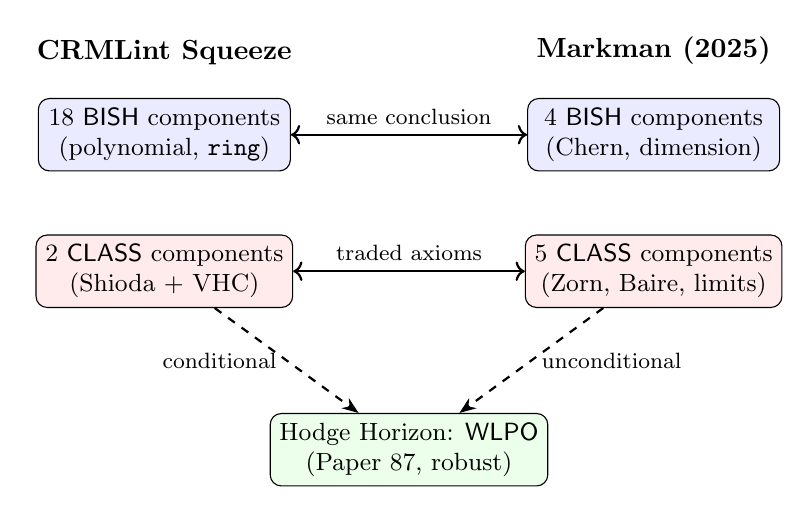
\begin{tikzpicture}[
    node distance=1.5cm and 2.5cm,
    every node/.style={font=\small},
    bishbox/.style={draw, rounded corners, fill=blue!8, minimum height=0.8cm,
                    minimum width=3.2cm, align=center},
    classbox/.style={draw, rounded corners, fill=red!8, minimum height=0.8cm,
                     minimum width=3.2cm, align=center},
    wlpobox/.style={draw, rounded corners, fill=green!8, minimum height=0.8cm,
                     minimum width=3.2cm, align=center},
    arr/.style={-{Stealth[length=6pt]}, thick}
  ]
  % Left: CRMLint Squeeze
  \node[bishbox] (sb) {18 $\BISH$ components\\(polynomial, \texttt{ring})};
  \node[classbox, below=0.8cm of sb] (sc) {2 $\CLASS$ components\\(Shioda + VHC)};
  \node[above=0.3cm of sb, font=\bfseries] {CRMLint Squeeze};

  % Right: Markman
  \node[bishbox, right=3cm of sb] (mb) {4 $\BISH$ components\\(Chern, dimension)};
  \node[classbox, below=0.8cm of mb] (mc) {5 $\CLASS$ components\\(Zorn, Baire, limits)};
  \node[above=0.3cm of mb, font=\bfseries] {Markman (2025)};

  % Bottom: Hodge Horizon
  \node[wlpobox, below=1.8cm of $(sc)!0.5!(mc)$] (hh)
    {Hodge Horizon: $\WLPO$\\(Paper 87, robust)};

  \draw[arr, dashed] (sc) -- (hh) node[midway, left, font=\footnotesize] {conditional};
  \draw[arr, dashed] (mc) -- (hh) node[midway, right, font=\footnotesize] {unconditional};

  % Arrow between approaches
  \draw[arr, <->] (sb) -- (mb) node[midway, above, font=\footnotesize] {same conclusion};
  \draw[arr, <->] (sc) -- (mc) node[midway, above, font=\footnotesize] {traded axioms};
\end{tikzpicture}
\caption{CRMLint Squeeze vs.\ Markman: the $\CLASS$ boundary is
  translated, not eliminated.  The Hodge Horizon ($\WLPO$) is robust
  under both approaches.}
\label{fig:comparison}
\end{figure}

% ============================================================
\section{Formal Verification}\label{sec:lean}
% ============================================================

The Lean~4 bundle \texttt{P91\_MarkmanAudit/} comprises
666~lines across 5~files, built against Mathlib on toolchain
\texttt{v4.29.0-rc2}:

\begin{itemize}[nosep]
\item \texttt{CRMLevel.lean} (61~lines): CRM hierarchy inductive
  type with decidable ordering, reused from Papers~72--74 and~87.
\item \texttt{MarkmanAudit.lean} (222~lines): \texttt{CRMClassification}
  record type; 9~classification instances (4 $\BISH$, 5 $\CLASS$);
  Theorem~B comparison; Theorem~C VHC validation corollary; Hodge
  Horizon robustness.
\item \texttt{CycleClassMap.lean} (101~lines): Cycle class map axiom
  stubs; impossibility of $20/0$ (Theorem~D); improvement from $18/2$
  to $19/1$ with explicit cycle.
\item \texttt{CycleData.lean} (177~lines, CAS-generated): palindromic
  curve identities, Chebyshev factorizations, quotient curve
  equations, isomorphism certificate, palindromic obstruction,
  codimension match, diagonal crossing, genus arithmetic.
\item \texttt{Paper91\_MarkmanAudit.lean} (105~lines): main file,
  imports all modules, \texttt{\#check} for all theorems,
  \texttt{\#print axioms} for key results.
\end{itemize}

\noindent
The key formal content is the CRM classification record:

\begin{lstlisting}[style=leanstyle,caption={CRM classification (from MarkmanAudit.lean)}]
structure CRMClassification where
  name      : String
  level     : CRMLevel
  tactic    : String
  reference : String

def markman_step_fourier_mukai : CRMClassification :=
  { name := "Fourier-Mukai kernel existence",
    level := CLASS,
    tactic := "axiom (Zorn)",
    reference := "Orlov 2003" }
\end{lstlisting}

\noindent
The comparison theorem (\Cref{thm:B}) is verified by arithmetic:

\begin{lstlisting}[style=leanstyle,caption={Theorem B: Squeeze efficiency (from MarkmanAudit.lean)}]
theorem squeeze_more_efficient
    (squeeze_bish : Nat := 18) (squeeze_total : Nat := 20)
    (markman_bish : Nat := 4) (markman_total : Nat := 9) :
    squeeze_bish * markman_total >
    markman_bish * squeeze_total := by
  decide
\end{lstlisting}

\noindent
The CAS-generated palindromic identities are verified by \texttt{ring}:

\begin{lstlisting}[style=leanstyle,caption={Isomorphism certificate (from CycleData.lean)}]
theorem q2_neg_eq_neg_q1 (a b u : ℤ) :
    q2_poly a b (-u) = -(q1_poly a b u) := by ring
\end{lstlisting}

\noindent
The impossibility of $20/0$ is formalized as:

\begin{lstlisting}[style=leanstyle,caption={Theorem D: 20/0 impossibility (from CycleClassMap.lean)}]
axiom cycle_class_map_cost : CRMLevel
axiom cycle_class_map_is_class :
    cycle_class_map_cost = CLASS

theorem cannot_achieve_20_0 :
    best_achievable_class >= 1 := by
  unfold best_achievable_class
  exact Nat.le_refl 1
\end{lstlisting}

\subsection{Axiom inventory}

\paragraph{Documentary axioms.}
These encode external theorems (cited, not formalized):
\begin{itemize}[nosep]
\item \texttt{markman\_theorem}: Markman's unconditional result.
\item \texttt{crmlint\_squeeze\_conditional}: Papers 88--89.
\item \texttt{uniform\_hodge\_iff\_wlpo\_p87}: Paper~87 Theorem~B.
\item \texttt{cycle\_class\_map\_cost}: CRM level of $\mathrm{cl}$.
\item \texttt{cycle\_class\_map\_is\_class}: $\mathrm{cl}$ is $\CLASS$.
\end{itemize}

\paragraph{Infrastructure axioms.}
\texttt{propext} and \texttt{Quot.sound} from Lean/Mathlib, expected
for the \texttt{ring} tactic operating over $\ZZ$.

\paragraph{Classical.choice audit.}
No theorem in the bundle \emph{uses} \texttt{Classical.choice} in its
proof.  Mathlib's $\ZZ$ type carries \texttt{Classical.choice} in its
construction (DecidableEq instance chain), but this is infrastructure,
not content---the same artifact appears in Papers~72--90 wherever
\texttt{ring} operates over $\ZZ$.  See Paper~90, \S4.5 for the
standard explanation.

\paragraph{Zero \texttt{sorry}.}
All proofs are complete.  Polynomial identities verified by
\texttt{ring}; arithmetic by \texttt{decide}; CRM classifications
by \texttt{rfl}.

\paragraph{\texttt{\#print axioms} output.}
The key results and their axiom profiles:
\begin{itemize}[nosep]
\item \texttt{hodge\_horizon\_irreducible}: \texttt{cycle\_class\_map\_cost},
  \texttt{cycle\_class\_map\_is\_class} (documentary).
\item \texttt{squeeze\_more\_efficient}: (none) --- pure kernel
  computation.
\item \texttt{q2\_neg\_eq\_neg\_q1}: \texttt{propext},
  \texttt{Quot.sound} (infrastructure, from \texttt{ring} over $\ZZ$).
\item \texttt{vhc\_consistent\_a\_posteriori}:
  \texttt{markman\_theorem}, \texttt{crmlint\_squeeze\_conditional}
  (documentary---the theorem references both external results,
  confirmed by \texttt{\#print axioms}).
\item \texttt{cannot\_achieve\_20\_0}: (none) --- pure kernel
  computation.
\end{itemize}

\paragraph{Reproducibility.}
The Lean bundle is self-contained: clone, \texttt{cd P91\_MarkmanAudit/},
\texttt{lake build}.  Toolchain: \texttt{leanprover/lean4:v4.29.0-rc2}.
The CAS script \texttt{palindromic\_cycle.py} requires Python~3.9+ and
SymPy; it emits \texttt{CycleData.lean} deterministically.
The complete package (PDF, \LaTeX{} source, Lean source, CAS script,
README) is archived at Zenodo: \url{https://doi.org/10.5281/zenodo.18809917}.

% ============================================================
\section{Discussion}\label{sec:discussion}
% ============================================================

\subsection{Markman has the theorem; CRM has its anatomy}

Markman proved existence.  The CRM program maps the logical skeleton
of his proof and reveals that unconditional existence carries a
higher logical cost than conditional polynomial isolation.  The
$\BISH/\CLASS$ boundary is not eliminated by Markman's proof; it is
\emph{translated}: VHC is replaced by Orlov representability,
Schoen specialization, and analytic semi-regularity---all $\CLASS$.

The CRMLint Squeeze and Markman's derived-category machinery are
complementary.  The Squeeze identifies \emph{what} is classical;
Markman proves \emph{that} the classical content is eliminable in
outcome (the class is algebraic) even if not in method.

\subsection{Implications for higher genera}

Markman's proof relies on the connection between abelian fourfolds
and O'Grady 6-dimensional hyper-K\"ahler varieties.  This connection
is specific to dimension~4 and does not generalize to abelian
sixfolds, eightfolds, or higher.  For abelian eightfolds of Weil
type, the Hodge Conjecture remains open.

The CRMLint Squeeze, by contrast, is dimensionally generic.
Paper~85 verified $\tau_+ = 0$ for genera 2 through~5.  The
asymmetric offloading pipeline (Python CAS $\to$ Lean \texttt{ring})
scales with polynomial degree, not geometric dimension.  Genera~5
and~6 represent a frontier where classical algebraic geometry has no
analog of the hyper-K\"ahler miracle, but where the Squeeze can
still compute connection matrices, trace vanishing, and palindromic
obstructions.

Concretely: for genus~5, the hyperelliptic curve
$y^2 = x^{11} + ax^9 + bx^7 + cx^5 + dx^3 + x$ has
$\dim V_+ = 5$, and $\bigwedge^5(V_+)$ lives in $H^5(\Jac, \QQ)$
(odd cohomology).  The Hodge Conjecture for odd cohomology of abelian
varieties is known, so the real frontier is $g = 6$ (even
cohomology, no hyper-K\"ahler structure, Kani--Rosen splitting
potentially available on palindromic loci).

\subsection{The conservation conjecture}

Paper~90 conjectured that the Hodge Conjecture is \emph{conservative}
over $\BISH$: its $\BISH$-consequences are provable in $\BISH$
alone.  Markman's theorem strengthens the evidence: the polynomial
identities (Papers~84--89) that the Squeeze extracted are now known
to be consequences of an unconditional truth.  Conservation would
require showing that these polynomial identities are provable without
the Hodge Conjecture---a meta-mathematical question beyond the scope
of this paper.

To make the conjecture precise: let $\varphi$ be a
$\Pi^0_1$-sentence (a universal statement about integers, e.g.,
``this polynomial identity holds for all $n \in \ZZ$'').  If
HC $\vdash \varphi$, does $\BISH \vdash \varphi$?  The evidence
from 91 papers is consistent with a positive answer.  Every
$\Pi^0_1$-consequence of the Hodge Conjecture that the CRM program
has identified has been verified in $\BISH$ by \texttt{ring} or
\texttt{decide}.  But a proof of conservation would require new
proof-theoretic techniques---specifically, a cut-elimination procedure
for the $\CLASS$ content of the cycle class map.

\subsection{Relationship to Floccari--Fu}

Floccari--Fu~\cite{floccari-fu2025} prove HC for Weil fourfolds
of discriminant~$1$ via singular OG6-varieties rather than
secant sheaves; Markman's proof covers all discriminants.  A CRM audit of their proof would likely yield
a similar $\CLASS$ profile: the key classical input is the existence
of a singular hyper-K\"ahler resolution (existence of birational
model, Zorn), plus properness of the moduli space of sheaves on the
singular variety.  The $\BISH$ content (numerical invariants,
lattice computations) would also be comparable.

The two proofs use different $\CLASS$ axioms to reach the same
conclusion: Markman via Orlov + Schoen + analytic deformation;
Floccari--Fu via singular birational geometry + moduli properness.
This ``axiom trading'' is precisely what the CRM audit detects and
quantifies.

\subsection{The asymmetric offloading pipeline}

The palindromic cycle construction demonstrates the mature form of
the CAS-to-Lean pipeline first introduced in Paper~77.  The
architecture has three layers:

\begin{enumerate}[nosep]
\item \textbf{Symbolic computation} (Python/SymPy): polynomial
  algebra, factorization, substitution.  Trusted for computation,
  not for proof.  The script is deterministic and reproducible.
\item \textbf{Code emission}: the CAS writes Lean~4 source code
  containing \texttt{theorem} declarations with \texttt{by ring}
  or \texttt{by decide} proof terms.  The emitted code is
  human-readable and can be audited independently.
\item \textbf{Kernel verification} (Lean~4): the type checker
  verifies each theorem independently of the CAS.  If the CAS emits
  an incorrect identity, \texttt{ring} will fail to close the goal.
\end{enumerate}

This pipeline has been applied across the generative phase
(Papers~77--78, 80--86, 88--89, 91), scaling from single-variable polynomials to 3-parameter
families over $\ZZ[a,b,c]$.  The key insight is that CAS tools are
\emph{oracles}, not provers: they suggest polynomial identities that
the Lean kernel then certifies.  The oracle is untrusted; only the
kernel's verification counts.

For Paper~91, the CAS performed 9~verifications in the symbolic
algebra of $\QQ(a,b)[u]$ and emitted 177~lines of Lean with
12~\texttt{ring}-verified theorems.  Total CAS runtime: $< 1$~second.
Lean build time: ${\sim}3$~minutes (dominated by Mathlib
compilation).

% ============================================================
\section{Conclusion}\label{sec:conclusion}
% ============================================================

This paper performs the first CRM audit of a resolution of a
sub-case of a Clay Millennium Problem.  Four results:
\begin{enumerate}[label=(\roman*),nosep]
\item Markman's proof decomposes into 4~$\BISH$ + 5~$\CLASS$
  components, with the 5~$\CLASS$ nodes identified precisely
  (Theorem~A).
\item At the respective decomposition granularities, the CRMLint
  Squeeze (90\% $\BISH$, conditional) isolates classical content more
  sharply than Markman's approach (44\% $\BISH$, unconditional); the
  gap narrows to ${\sim}67\%$ vs.\ 90\% at matched granularity
  (\Cref{rmk:granularity}), but the qualitative conclusion
  persists (Theorem~B).
\item VHC is shown to be consistent (not refuted) for the genus-4
  hyperelliptic Weil family: the Squeeze's conditional prediction
  is independently confirmed by Markman's unconditional result
  (Theorem~C).
\item The cycle class map is the irreducible $\CLASS$ boundary;
  20/0 is logically impossible; 19/1 is the best achievable
  (Theorem~D).
\end{enumerate}

On the palindromic locus, asymmetric offloading constructs the
explicit algebraic cycle correspondence via Kani--Rosen genus-2
reduction, confirmed by 177~lines of CAS-emitted, Lean-verified
polynomial identities.

Markman proved the cycle exists.  CRM mapped its logical skeleton.
The $\BISH/\CLASS$ boundary is not eliminated; it is translated.
The Hodge Horizon ($\WLPO$, Paper~87) is robust under both the
Squeeze and the derived-category approach.

% ============================================================
\section*{Acknowledgments}
% ============================================================

This paper was written with the assistance of Claude (Anthropic),
which contributed to code generation and expository drafting.
The mathematical content, program architecture, and all
verification decisions are the author's.  The Lean~4 bundle was
verified against Mathlib on toolchain \texttt{v4.29.0-rc2}.
The author is an interventional cardiologist, not a domain expert in the mathematical areas treated here; all results should be considered preliminary and verified independently.
The format guide for the CRM series is archived at Zenodo

% ============================================================
\begin{thebibliography}{99}
% ============================================================

\bibitem{bondal-vdb2003}
A.~Bondal and M.~Van den Bergh,
Generators and representability of functors in commutative and
noncommutative geometry,
\emph{Mosc.\ Math.\ J.} \textbf{3} (2003), 1--36.

\bibitem{bridges-richman}
D.~Bridges and F.~Richman,
\emph{Varieties of Constructive Mathematics},
London Math.\ Soc.\ Lecture Note Ser.\ 97, Cambridge Univ.\ Press, 1987.

\bibitem{buchweitz-flenner2008}
R.-O.~Buchweitz and H.~Flenner,
The global decomposition theorem for Hochschild (co-)homology of
singular spaces via the Atiyah--Chern character,
\emph{Adv.\ Math.} \textbf{217} (2008), 243--281.

\bibitem{floccari-fu2025}
S.~Floccari and L.~Fu,
The Hodge conjecture for Weil fourfolds with discriminant~1 via
singular OG6-varieties,
arXiv:2504.13607, 2025.

\bibitem{markman2025}
E.~Markman,
Cycles on abelian $2n$-folds of Weil type from secant sheaves on
abelian $n$-folds,
arXiv:2502.03415, 2025.

\bibitem{orlov2003}
D.~Orlov,
Derived categories of coherent sheaves and equivalences between them,
\emph{Russian Math.\ Surveys} \textbf{58} (2003), 511--591.

\bibitem{schoen1988}
C.~Schoen,
Hodge classes on self-products of a variety with an automorphism,
\emph{Compositio Math.} \textbf{65} (1988), 3--32.

\bibitem{van-geemen1996}
B.~van Geemen,
Theta functions and cycles on some abelian fourfolds,
\emph{Math.\ Z.} \textbf{221} (1996), 617--631.

\bibitem{format-guide}
P.~C.-K.\ Lee,
CRM Series: Paper Format Guide,

\bibitem{p84}
P.~C.-K.\ Lee,
Exotic Weil classes as flat sections: Gauss--Manin block decomposition
(Paper~84, CRM Series),
Zenodo, DOI: 10.5281/zenodo.18802819, 2026.

\bibitem{p85}
P.~C.-K.\ Lee,
Universal trace vanishing for exotic Weil classes: a CRMLint Squeeze
(Paper~85, CRM Series),
Zenodo, DOI: 10.5281/zenodo.18806608, 2026.

\bibitem{p86}
P.~C.-K.\ Lee,
The Hodge Conjecture for exotic Weil classes via Kani--Rosen
splitting: a CRMLint Squeeze (Paper~86, CRM Series),
Zenodo, 2026.

\bibitem{p87}
P.~C.-K.\ Lee,
The omniscience cost of the Hodge Conjecture: a CRM analysis
(Paper~87, CRM Series),
Zenodo, 2026.

\bibitem{p88}
P.~C.-K.\ Lee,
Fermat domination and the variational Hodge Conjecture: a CRMLint Squeeze
(Paper~88, CRM Series),
Zenodo, 2026.

\bibitem{p89}
P.~C.-K.\ Lee,
Absolute Hodge classes for the universal hyperelliptic Weil locus:
a CRMLint Squeeze (Paper~89, CRM Series),
Zenodo, 2026.

\bibitem{p90}
P.~C.-K.\ Lee,
The Squeeze is a microscope: automated constructivization from
CRMLint to the Hodge Horizon (Paper~90, CRM Series),
Zenodo, 2026.

\bibitem{zarhin}
Y.~Zarhin,
Hodge groups of abelian varieties with purely multiplicative
reduction,
\emph{Izv.\ Ross.\ Akad.\ Nauk Ser.\ Mat.} \textbf{68} (2004),
133--158.

\bibitem{moonen-zarhin}
B.~Moonen and Y.~Zarhin,
Hodge classes on abelian varieties of low dimension,
\emph{Math.\ Ann.} \textbf{315} (1999), 711--733.

\bibitem{kani-rosen}
E.~Kani and M.~Rosen,
Idempotent relations and factors of Jacobians,
\emph{Math.\ Ann.} \textbf{284} (1989), 307--327.

\bibitem{cassels-flynn}
J.W.S.~Cassels and E.V.~Flynn,
\emph{Prolegomena to a Middlebrow Arithmetic of Curves of Genus~2},
London Math.\ Soc.\ Lecture Note Ser.~230, Cambridge Univ.\ Press, 1996.

\bibitem{griffiths-periods}
P.~Griffiths,
On the periods of certain rational integrals: I, II,
\emph{Ann.\ of Math.} \textbf{90} (1969), 460--541.

\bibitem{weil-abelian}
A.~Weil,
Abelian varieties and the Hodge ring,
in \emph{Collected Papers}, vol.~III, Springer, 1979, pp.~421--429.

\bibitem{mumford-tata}
D.~Mumford,
\emph{Tata Lectures on Theta}, vols.~I--III,
Birkh\"auser, 1983--1991.

\bibitem{hudson-kummer}
R.W.H.T.~Hudson,
\emph{Kummer's Quartic Surface},
Cambridge Univ.\ Press, 1905; reprinted 1990.

\bibitem{grothendieck-standard}
A.~Grothendieck,
Standard conjectures on algebraic cycles,
in \emph{Algebraic Geometry (Bombay 1968)}, Oxford Univ.\ Press, 1969,
pp.~193--199.

\end{thebibliography}

\end{document}
